\subsection{Homogeneous vs Inhomogeneous}
We used a fixed set of parameters to compare the homogeneous and inhomogeneous HMM algorithms, $L=100$, $p=0.80$, $e=0.10$, and $N=10$. A plot of the likelihood of the two methods is given in Figure \ref{fig:tIndep_vs_tDep}. We observe that the inhomogeneous HMM consistently converges to a greater likelihood than the homogeneous HMM. However, we also observe that the higher likelihood is associated with less accumulated entropy at locations of inference error. Because the goal is to develop heuristics for identifying errors in the sequence inference, this may prove less valuable. 

\begin{figure}[h!]
\centering
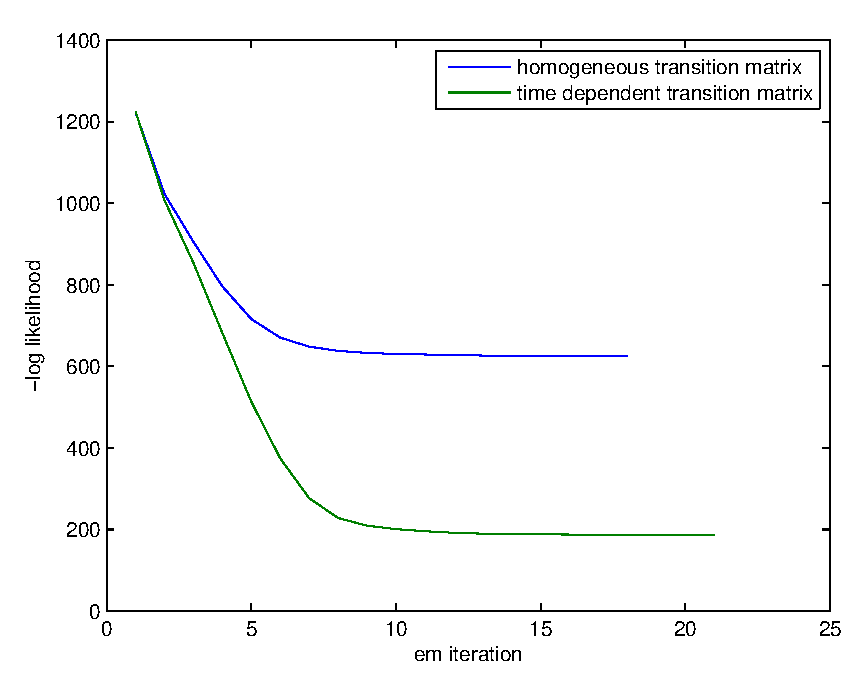
\includegraphics[width=.5\textwidth]{fig/homog_vs_tDep_L100_p80_e10_N10}
\caption{Comparing homogeneous and inhomogeneous likelihood convergence}
\label{fig:tIndep_vs_tDep}
\end{figure}

%\section{Sampling}
%The problem has substantial l
%It has become clear that due to the presence of a substantial number of local minima, sampling will be necessary. Here we present a rough outline of a plan of attack of introducing a sampling step into our inference routine.
%\subsection{Method 1}
%Integrate sampling into the EM algorithm. It was initially suggested to perform a forward-smooth backward-sample type algorithm. This has yet to be coded.
%\subsection{Method 2}

\subsubsection{Homogeneous vs Inhomogeneous}
Most HMM algorithms assume a time-independent transition matrix, which is what goes into each step of the forward-backward algorithm. Not necessarily the case here. Ran experiments with a time-dependent transition matrix. Updates to the transition matrix were obtained by calculating $\xi$ in the range $2:T$ and summing over the upper diagonal elements. This gives the probability that a forward transition occured at that time step. 


%%% ADDITIONAL NOTES

\section{Additional Notes}

\subsection{Limits on Inference Accuracy}
The accuracy of the present inference algorithm is limited by the read error rate, $e$. To explore this, we generated synthetic data over a range of parameter values and measured the entropy of perfect inference. That is, we took the hidden states $\mathbf{Z}$ as observed, constructed the sequence estimate $S$, and measured the entropy of this estimate. Results are shown in attached figures. A few interesting things can be seen. One, the inference entropy increases with an increasing read number. Two, entropy often rises smoothly with varying parameters. It's highly likely I can derive a formula for the expected entropy of perfect inference given a set of parameters as some function of the expected number of errors per 

To improve further, it will be necessary to modify our model to include an additional latent variable representing errors in individual base reads. We can imagine doing this across multiple reads using a type of consensus model.

\subsection{Jackknife Estimation and Multiple Sequence Alignment}
Examining the behavior of the inference algorithm average over multiple reads, it is often apparent that a given individual read will tend to drive the inference towards a specific local minimum of the system. To attempt to smooth out this effect, it was proposed that less biased estimates of the true sequence be constructed by a jackknife estimation process. Here, we generate data as usual, a set of $N$ reads of a given sequence. Rather than feeding the entire set of reads into the inference algorithm, we construct jackknifed subsamples via a 'hold-one-out' scheme The output of this process is a set of $N$ sequence estimates. 

\subsection{Path Counting}
In this section, we use a \emph{lattice path} construction to provide combinatorial formulas for statistics of interest in a random walk, subject to the constraints of DNA moving through a nanopore sequencer. In a lattice path, we represent a one-dimensional random walk on a two-dimensional lattice. A walk begins at the origin, and moves one point to the right for every forward (+1) transition, and one point up for every backward (-1) transition. This provides an alternate characterization of a given random walk in terms of the number of forward transitions, $F$, and the number of backward transitions $B$. In a random walk of known length $T$ on a sequence of known length $L$, these quantities will be related by
\begin{equation}
F+B = T-1
\end{equation}
\begin{equation}
F-B = L-1
\end{equation}
or,
\begin{equation}
F = \frac{1}{2}(T+L) - 1
\end{equation}
\begin{equation}
B = \frac{1}{2}(T-L)
\end{equation}
The total number of paths that take us from the $l=1$ to $l=L$ in $T-1$ steps will be given by
\begin{equation}
L = \binom{F+B}{F} = \frac{(F+B)!}{F!B!}
\end{equation}
However, we have constraints on the number of valid paths, which can be elegantly visualized using the lattice path construction and the \emph{reflection principle}. The argument is as follows: consider a path that makes a first legal to the right, and at a later time hits the constraint, at which point it becomes an illegal path. Consider a reflection of that path
\begin{equation}
L = \binom{F+B-1}{F-1} - \binom{F+B-1}{B-1}
\end{equation}
Dividing this by the total path count $\binom{F+B}{F}$ gives the probability that an arbitrary path is legal
\begin{equation}
p(\mathrm{legal path}) = \frac{F-B}{F+B}
\end{equation}

%This is the celebrated \emph{ballot theorem}, originally derived in the late Nineteenth century as an expression for the probability that in an election, votes for one candidate (F) will always exceed those of the second candidate (B). Hence we have an expression for the total number of paths that do not hit the line $y=x$ except at the origin. Next we apply the restriction that a given sequence does not exit the sequence early. Again, we know $T$ and $L$. So anyways, if we wanted to sample a path


On its own this construction is of only mild utility, primarily because of its uncomputatibility. But the same construction allows us to get a variety of \emph{rank order statistics} that allow us to make useful statements about probabilities of random walks.

\begin{equation}
L = \binom{F+B-1}{F-1} - 2\binom{F+B-1}{B-1} + \left(\frac{F-B}{F+B}\right)^2\binom{F+B}{F}
\end{equation}
